% !TEX TS-program = LuaLaTeX
\documentclass[10pt, oneside, a4paper]{article}

\usepackage[T1]{fontenc}
\usepackage{lmodern}
\usepackage{xcolor}
    \definecolor{gray} {HTML}{363636}
    \definecolor{red}  {HTML}{950009}
    \definecolor{green}{HTML}{0E610A}
    \definecolor{blue} {HTML}{020069}
\usepackage{fontspec}
    \setsansfont{Arial}
\usepackage{amsmath}
\usepackage{titlesec}
    \titleformat*{\section}      {\color{gray}\large\bfseries\sffamily}
    \titleformat*{\subsection}   {\color{gray}\large\bfseries\sffamily}
    \titleformat*{\subsubsection}{\color{gray}\large\bfseries\sffamily}
\usepackage{geometry}
    \geometry{scale={0.75,0.85}}
\usepackage{siunitx}
    \sisetup{locale=FR}
    \sisetup{math-micro=\text{µ},text-micro=µ} % fix
\usepackage{graphicx}
\usepackage{caption}
    \captionsetup{labelfont={bf,sf,color=gray}}
\usepackage{pdfpages}
\usepackage{caption}

\usepackage{fancyhdr}
\pagestyle{fancy}
\fancyhead[R]{}
\fancyfoot[L]{Thomas Anizet}
\fancyfoot[C]{}
\fancyfoot[R]{\thepage}


% Keep lasts
\usepackage[french]{babel}
    \frenchsetup{SmallCapsFigTabCaptions=false}
\usepackage[expansion]{microtype}
\usepackage[luatex, backref]{hyperref}
    \hypersetup{unicode, colorlinks, breaklinks, urlcolor=red,
                bookmarksopen, bookmarksnumbered}

\renewcommand{\UrlFont}{\small}
\renewcommand{\arraystretch}{1.1}
\setlength{\parskip}{2mm}

\begin{document}


%%%%%%%%%%%%%%%%%%%%%%%% Table des matières
\tableofcontents
\newpage

%%%%%%%%%%%%%%%%%%%%%%%% Introduction

\phantomsection
\section*{Introduction}
\addcontentsline{toc}{section}{Introduction}

Candidat "Officier de carrière" à l’\textbf{\textit{École Royale Militaire}} (ERM), je suis actuellement ma formation académique à l’\textbf{\textit{École Centrale des Arts et Métiers}} (ECAM) en option électronique. \\ \\
Durant notre 2ème année de Master, les étudiants doivent réaliser un stage d’immersion en entreprise d’une durée de 6 semaines. Ce stage consiste, entre autres, à s’insérer dans une entreprise afin d’y découvrir différents aspects tels que l’organisation générale d’une entreprise, son management, son contexte social, son insertion économique, ses aspects techniques et ses produits. Il a également pour but de se familiariser au travail quotidien de l’ingénieur en participant à diverses activités. \\ \\
Ayant réalisé mon stage de 3ème Bachelier chez \textbf{\textit{AIRBUS DS SLC}} sur le site de Diegem et de Elancourt, il était important pour moi de saisir la chance et l’opportunité de découvrir une nouvelle entreprise renommée à travers le monde. C'est ainsi que je décidai de réaliser mon stage chez \textit{\textbf{THALES} Telecommunications Belgium} sur le site de Tubize. 

\newpage

%%%%%%%%%%%%%%%%%%%%%%%% Partie 1 - Environnement de stage %%%%%%%%%%
\section{Environnement de stage}
Cette section a pour objectif de décrire l'entreprise à différents points de vue. Tout d'abord, une description de la structure de l'entreprise (dont l'équipe dans laquelle se trouve le stagiaire) et de ses objectifs est reprise. Ensuite, sont détaillées succontement la gestion de production mais aussi la gestion marketing, la gestion financière et la gestion des ressources humaines. Enfin, un descriptif de la cellule qualité clôturera ce premier point.

\subsection{Structure de l'entreprise}
C'est donc chez \textbf{\textit{Thales}} \textit{Telecommunication Belgium} que je me suis rendu pour réaliser mon stage d'immersion en entreprise. 

\subsection{Objectifs de l'entreprise}


\subsection{Equipe du stagiaire}


\subsection{Gestion de production}


\subsection{Gestion marketing}


\subsection{Gestion financière}


\subsection{Gestion des ressources humaines}


\subsection{Politique QHSE}


\newpage
%%%%%%%%%%%%%%%%%%%%%%%% Partie 2 - Objectifs du stage %%%%%%%%%%%%%
\section{Objectifs du stage}
\label{sec:objectifs}

L'objectif de ce stage était d'introduire l'ensemble des notions élémentaires, nécessaires pour la réalisation du \textit{Travail de Fin d'Étude} (TFE). Ce travail de fin d'étude qui allait se poursuivre durant 6 mois à compter du mois de Novembre 2018. Dans un premier temps, une définition des notions théoriques est abordée. Ensuite, un exemple ou une simulation est mise en oeuvre afin d'appuyer le concept théorique.\\ \\
La liste ci-dessous reprend l'ensemble des objectifs fixés et réalisés durant les 6 semaines de stage : 
\begin{description}
\item[1. Notions  de chiffrement et de \textit{Side-Channel Attacks} (attaques par canal auxiliaire)] 
\item[2. L'algorithme AES (\textit{Advanced})]
\item[3. Simulation d'un tracé et d'une attaque par canal auxiliaire sur MATLAB] 
\item[4. Notions de statistiques et de t-test] 
\item[5. Simulation d'un t-test sur MATLAB] 
\end{description}
Ces différents objectifs sont décrits dans la section \ref{sec:Projet} \textit{"Projet du stage"}.

%%%%%%%%%%%%%%%%%%%%%%%% Partie 3 - Projet du stage %%%%%%%%%%%%%
\section{Projet du stage}
\label{sec:Projet}

Cette section décrit l'ensemble des objectifs, cités à la section \ref{sec:objectifs}, fixés pour le stage. 

%%%% PARTIE 3.1
\subsection{Notions  de chiffrement et de \textit{Side-Channel Attacks}}

Les systèmes de sécurité modernes utilisent des algorithmes de chiffrement pour assurer la disponibilité, la confidentialité et l'intégrité de données. Ces algorithmes de chiffrement sont en réalité des fonctions mathématiques qui prennent typiquement : 
\begin{itemize}
\item  2 paramètres en entrée : un \textbf{\textit{message clair}} (nommé \textit{plaintext} en anglais) et une \textbf{\textit{clé de chiffrement}} (nommé \textit{key} en anglais).
\item 1 paramètre en sortie : le \textbf{\textit{message chiffré}} (nommé \textit{ciphertext} en anglais). \\
\end{itemize}
Le procédé transformant les données claires en entrée en données chiffrées en sortie est appelé le \textbf{\textit{chiffrement}}.
Ce procédé est réalisé grâce à un \textbf{\textit{algorithme de chiffrement}} utilisant une clé de chiffrement et diverses opérations mathématiques. Il est important de préciser que tous les détails décrivant le fonctionnement d'un algorithme sont disponibles publiquement, seule la clé de chiffrement doit rester secrète. 

La figure \ref{fig:chiffrement} ci-dessous présente le principe de fonctionnement d'un algorithme de chiffrement.

\begin{figure}[htbp]
    \centering
    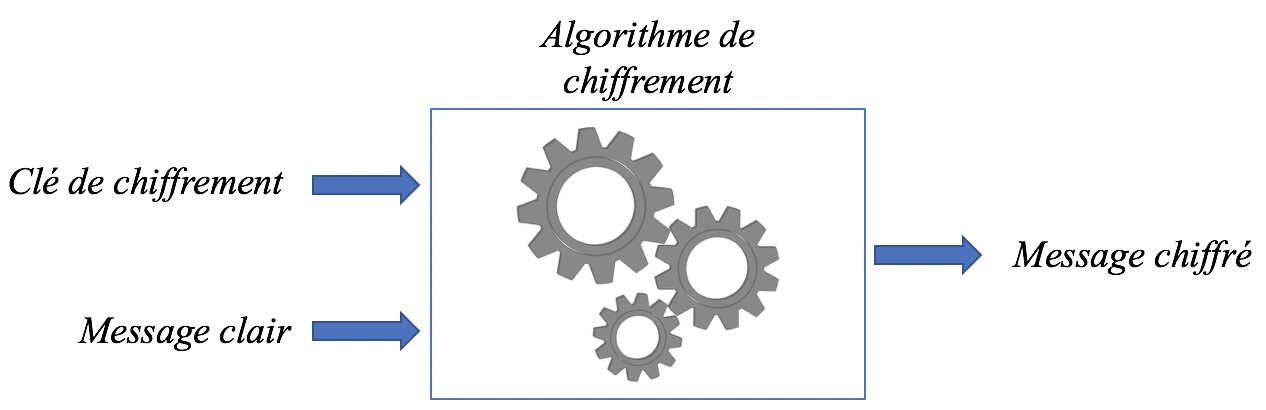
\includegraphics[width=0.7\textwidth]{image/chiffrement}
    \caption{L'algorithme de chiffrement, caractérisé par diverses opérations mathématiques, utilise une clé de chiffrement en entrée pour chiffrer un message clair. Cela produit un message chiffré, non compréhensible pour une personne ne connaissant pas la clé de chiffrement.}
    \label{fig:chiffrement}
\end{figure}

Nous distinguons 2 types d'algorithmes de chiffrements : 
\begin{itemize}
\item \textbf{\textit{Chiffrement symétrique}} : Le chiffrement est dit symétrique lorsque le procédé de chiffrement (algorithme) utilise une seule clé, appelée \textit{clé secrète}. Par convention, ce type de chiffrement permet à la fois de chiffrer et de déchiffrer des messages à partir d'une seule et unique clé. Le désavantage de ce typer de chiffrement est que si une personne parvient à subtiliser la clé publique, elle sera en mesure de déchiffrer tout message qu'elle intercepte.  \\
\textit{Exemple} : L'algorithme AES.
\item \textbf{\textit{Chiffrement asymétrique}} : Le chiffrement est dit asymétrique lorsque le procédé de chiffrement (algorithme) utilise 2 clés : une \textit{clé publique} et une \textit{clé privée}. Par convention, la clé publique est la clé de chiffrement du message clair, elle peut être communiquée sans aucune restriction tandis que la clé privée est la clé de déchiffrement du message chiffré, elle ne doit être communiquée sous aucun prétexte. Le fonctionnement est le suivant : Avec une clé publique, l'expéditeur code, dans un algorithme de chiffrement donné, un message. Ce message, une fois transmis, ne pourra être déchiffré que par le destinataire, détenteur de la clé privée. \\
\textit{Exemple} : L'algorithme RSA. \\
\end{itemize}

Les figures \ref{fig:symétrique} et \ref{fig:asymétrique} ci-dessous présentent les principes de fonctionnement des chiffrements symétriques et asymétriques.

\begin{figure}[htbp]
    \centering
    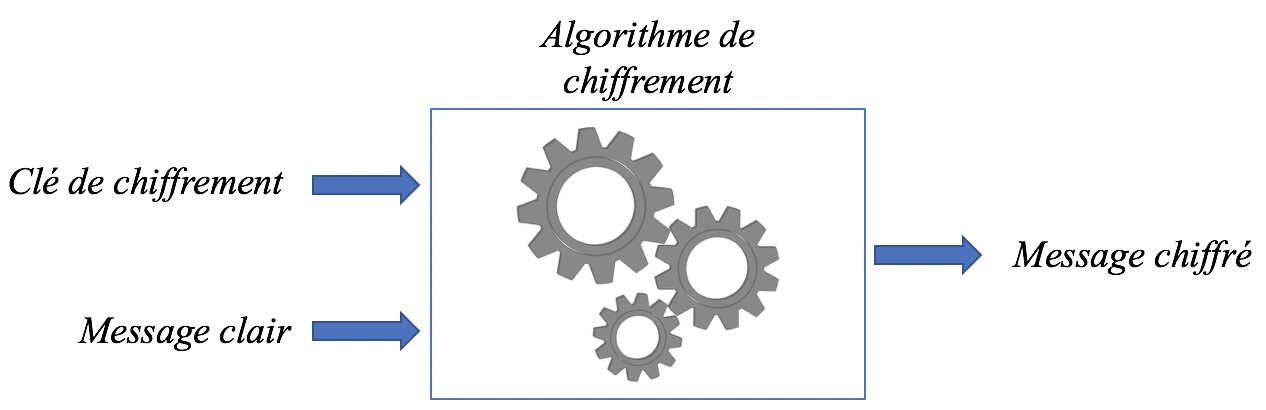
\includegraphics[width=0.7\textwidth]{image/chiffrement}
    \caption{Chiffrement symétrique : Une seule clé est utilisée pour chiffrer et déchiffrer les messages.}
    \label{fig:symétrique}
\end{figure}

\begin{figure}[htbp]
    \centering
    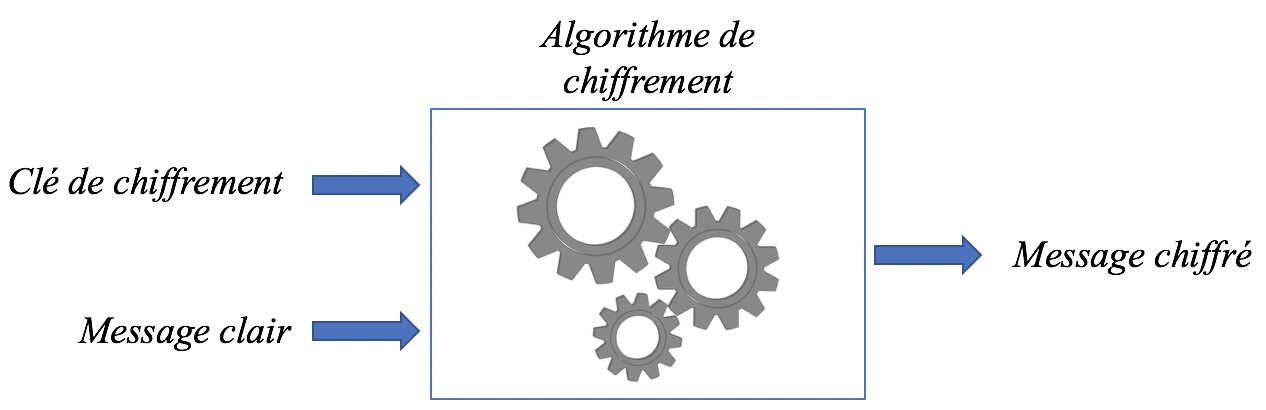
\includegraphics[width=0.7\textwidth]{image/chiffrement}
    \caption{Chiffrement asymétrique : Un clé publique est utilisée pour chiffrer le message et une clé privée est utilisée pour le déchiffrer.}
    \label{fig:asymétrique}
\end{figure}

\subsection{Algorithme AES}

\subsection{Simulation d'un tracé et d'une attaque par canal auxiliaire sur MATLAB}

Afin de bien assimiler les notions de \textit{side-channel attacks}, il m'a été demandé de réaliser une simulation sur MATLAB. La première phase de la simulation génère des traces sur base de l'algorithme AES. La seconde phase de la simulation est une attaque par canal auxiliaire. Plus précisément, cette attaque est réalisée sur un seul byte de donnée et se fait en sortie de la SBox. Ce type d'attaque est appelé CPA. Pour cette raison, seules les 2 premières étapes de l'algorithme AES sont nécessaires et seront donc simulées (\textit{AddRoundKey()}, \textit{SubBytes()}).


\subsection{Notions de statistiques et de t-test}

\subsection{Simulation d'un t-test sur MATLAB}


\newpage
%%%%%%%%%%%%%%%%%%%%%%%% Partie 4 - Conclusion %%%%%%%%%%%%%%%
\section{Conclusion}


\newpage
%%%%%%%%%%%%%%%%%%%%%%%% CREDITS %%%%%%%%%%%%%%%%%%%%
\pagebreak
\phantomsection
\section*{Crédits}
\addcontentsline{toc}{section}{Crédits}

\begin{itemize}
\item Figure~\ref{fig:sigmaDelta} provenant de :\\*
Le blog officiel de Texas Instrument :
\url{https://e2e.ti.com/blogs_/archives/b/precisionhub/archive/2015/01/21/delta-sigma-adc-basics-understanding-the-delta-sigma-modulator}

\item Figure~\ref{fig:classeD} provenant de :\\*
Par Yves-Laurent (Travail personnel) [GFDL (\url{http://www.gnu.org/copyleft/fdl.html}),
CC-BY-SA-3.0 (\url{http://creativecommons.org/licenses/by-sa/3.0/})], de Wikimedia Commons

\item Figure~\ref{fig:filtreLowpass} provenant de :\\*
Par Inductiveload (Travail personnel) [Public domain], de Wikimedia Commons

\item Figure~\ref{fig:filtreHighpass} provenant de :\\*
Par Toriicelli (Travail personnel) [Public domain], de Wikimedia Commons

\item Figure~\ref{fig:IntegPur} provenant de :\\*
Par Daniel Braun [GFDL (\url{http://www.gnu.org/copyleft/fdl.html}),
CC-BY-SA-3.0 (\url{http://creativecommons.org/licenses/by-sa/3.0/}) ou
CC BY 2.5 (\url{https://creativecommons.org/licenses/by/2.5})], de Wikimedia Commons
\end{itemize}

%%%%%%%%%%%%%%%%%%%%%%%% REFERENCES %%%%%%%%%%%%%%%%%%%%
\phantomsection
\addcontentsline{toc}{section}{Références}

\bibliographystyle{unsrt}
\bibliography{ampli-classe-d}

\end{document}
